\documentclass{article}
\usepackage{amsmath}
\usepackage{amssymb}
\usepackage{graphicx}
\usepackage{hyperref}
\usepackage[version=4]{mhchem}


\begin{document}
If the measures of two sides and the included angle of a triangle are \(7, \sqrt{50}\), and \(135^{\circ}\), respectively, find the measure of the segment joining the midpoints of the two given sides.\\
\centering
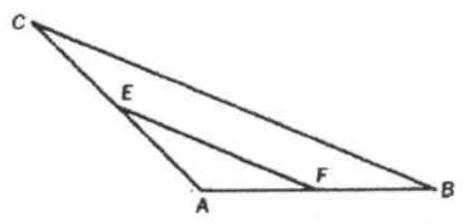
\includegraphics[width=\textwidth]{images/078.jpg}

Solution: \(\frac{13}{2}\).


Draw altitude \(C D\). Since \(\angle C A B=135, \angle D A C=45\), therefore, \(\triangle A D C\) is an isosceles right triangle. If \(A C=\sqrt{50}=5 \sqrt{2}\), then \(D A=\) \(D C=5\).\\
In \(\triangle D B C\), since \(D B=12\) and \(D C=5, B C=13\).\\
\centering
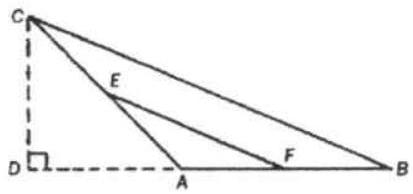
\includegraphics[width=\textwidth]{images/079.jpg}

Therefore, \(E F=\frac{1}{2} B C=\frac{13}{2}\).


\end{document}
